\documentclass[a4paper,12pt,oneside,openany,dvipdfmx]{jsbook}
\bibliographystyle{junsrt}
\usepackage{amsmath}
\usepackage{amsfonts}
\usepackage{bm}
\usepackage{graphicx}
\usepackage[hyphens]{url}
\usepackage{algorithm}
% \usepackage[noend]{algpseudocode}
% \usepackage{ascmac}
\usepackage{tikz}
\usetikzlibrary{bayesnet}

\makeindex
\setlength{\textwidth}{\fullwidth}
% \setlength{\textheight}{40\baselineskip}
\addtolength{\textheight}{\topskip}
% \setlength{\voffset}{-0.55in}
\newcommand{\argmax}{\mathop{\rm arg~max}\limits}
\newcommand{\argmin}{\mathop{\rm arg~min}\limits}
\newcommand{\average}[1]{\ensuremath{\langle#1\rangle} }
\renewcommand{\figurename}{Fig. }
\renewcommand{\tablename}{Table }

\title{
    平成31年度\\
    卒業論文\\
    複雑環境下でのロボット学習に向けた\\
    深層状態空間モデルを用いた映像予測
}
\author{
    平成32年2月\\
    指導教員 松尾豊教授\\
    \\
    東京大学工学部システム創成学科\\
    知能社会システムコース\\
    03-180961 近藤生也
}
\date{}
\begin{document}
\maketitle
\pagestyle{plain}
\setlength{\baselineskip}{22truept}
\frontmatter
\chapter*{概要}
\addcontentsline{toc}{chapter}{概要}
\label{chap:abstract}

近年,深層ニューラルネットワーク(DNN)を使用した機械学習手法の発展を背景としてロボットの制御方策を自ら学習させるロボット学習の研究が進んでいる.ロボット学習において未来の観測,特に自らの行動に対するフィードバックを適切に予測することは,より良い制御方策の獲得に繋がえる上,安全性の評価などに欠かせない.時間変化する環境のDNNを用いたモデル化手法として深層状態空間モデル(DSSM: Deep State Space Model)があり,これは昨今深層強化学習の分野で取り入れられているが,DSSMを用いて映像予測を学習することで良い環境の遷移モデルを獲得できることがわかっている.しかし現在一般的に使われているDSSMとその学習方法は各時刻の状態が低次元のベクトルで表現できるという仮定を暗に置いており,高次元な表現を仮定すると学習が進まず複雑な環境の予測問題にスケールさせる方法は自明でない.本研究ではまずこのような問題があることを実験的に指摘した上で,状態の表現に階層性を考えることでDSSMにより高次元な状態ベクトルを使っても学習が進むよう改善し,さらに低次元な状態ベクトルを用いた場合よりも良い表現が獲得できることを示す.評価実験では様々な物体が置かれた机上でのロボットマニピュレーションを題材にしたデータセットを用いてロボットの行動で条件付けた映像予測を行う.本研究では単純なDSSMをベースラインに設定し,提案手法の有効性を示した上で,研究の展望と社会応用の可能性について述べる.



% 近年,深層ニューラルネットワーク(DNN)を使用した機械学習手法の発展を背景としてロボットの制御方策を自ら学習させるロボット学習の研究が進んでいる.
% ロボット学習において未来の観測,特に自らの行動に対するフィードバックを適切に予測するよう学習することは,環境の遷移モデル(内部モデル)を獲得すること,そしてそれを用いたプランニングや行動結果の予測,安全性の評価などに欠かせない.
% 時間変化する環境のDNNを用いたモデルとして深層状態空間モデル(Deep State Space Model)があり,これは昨今深層強化学習の分野で取り入れられているが,深層状態空間モデルを用いて映像予測を学習することで内部モデルが獲得できるとされている\cite{Gregor2015}.
% しかし現在一般的に使われて深層状態空間モデルとその学習方法は各時刻の状態が低次元のベクトルで表現できるという仮定を暗に置いており,高次元な表現を仮定すると学習が進まず,複雑な環境の予測問題にスケールさせる方法は自明でない.

% 本研究ではまずこのような問題があることを実験的に指摘した上で,状態の表現に階層性を考えることで深層状態空間モデルにより高次元な状態表現を仮定できるように拡張し,低次元な表現を仮定した場合よりも良い表現が獲得できることを示す.評価実験では様々な物体が置かれた机上でのマニピュレーションを題材にしたデータセットを用いてロボットの行動で条件付けた映像予測を行う.単純な深層状態空間モデルをベースラインに設定し,提案手法の定性的・定量的な有効性を示す.
\setcounter{tocdepth}{2}
\tableofcontents
\listoffigures
\listoftables
\mainmatter
% \chapter{序論}
\label{chap:introduction}
\section{本研究の背景}
\subsection{ロボット学習と行動条件付き映像予測}
多様な環境で様々なタスクが遂行可能な汎用的なロボット(generalist robots)の開発はロボット工学の最重要課題の一つである\cite{escudero2015distance}.ロボットハードウェアの低価格化,汎用的なロボットソフトウェアの普及に加え,近年の急速な深層学習技術の発展を受けてロボットの制御方策を自ら学習させる{\bf ロボット学習}の研究が進んでおり,ロボットで遂行可能なタスクは着実に増えてきている.

ロボット学習において,将来予測,特に映像予測を明示的に学習することは,

\begin{itemize}
    \item ロボット自身が映像予測を用いた方策をたてることが可能になる
    \item 映像予測結果を人が評価することでロボットの行動を予め評価できる
\end{itemize}
という大きく二つの点からで重要であると言える.一点目の映像予測を用いた方策の例として,Hafnerら\cite{hafner2019planet}は,強化学習の問題設定において明示的に学習した映像予測モデルを用いることで行動系列をランダムにサンプリングして評価するような簡単なアルゴリズムで効率的なプランニングが可能であることを示した.二点目の映像予測を人が評価する例としてEbertらによる研究\cite{ebert2018visual}では学習した映像予測モデルを用いて,ロボットの操作によって予想される物体の移動の軌跡を確率分布として出力することができ,これを用いて人がロボットの行動の正しさを予め判断することができる.

このようにロボット学習における映像予測は重要であるが,映像予測だけを切り取って研究されることも多い.映像予測の中でも,ロボットの行動の結果として観測される映像を予測する問題設定を{\bf 行動条件付き映像予測}と呼び\cite{oh2015actionconditional}\cite{finn2016unsupervised}\cite{babaeizadeh2017stochastic},様々な研究がなされてきている.近年高精度な行動条件付き映像予測手法がいくつか提案されており,ロボット学習研究で扱うタスクの高度化を背景にしてこれらの映像予測手法をより複雑な問題設定に対して適用していきたいと考えられているが,いくつかの研究で既存の行動条件付き映像予測は上手く機能しない可能性があることがわかってきている.ただしここでいう「より複雑な問題設定」とは具体的には環境中に複数の操作対象の物体が隣接し合って置かれている場合,操作対象が布などの非剛体物である場合など,観測の時間変化に多数のパラメータが関与していたり,複雑な物理法則がはたらいているような問題設定を想定している.

\subsection{既存の行動条件付き映像予測手法の問題点}

行動条件付き映像予測手法は大きく{\bf 回帰型ニューラルネットワーク(RNN)ベースの手法}と{\bf 深層状態空間モデル(DSSM)ベースの手法}に分けられる.Hafnerら\cite{hafner2019planet}の研究など深層強化学習の問題で映像予測を明示的に行う場合は後者のDSSMベースの手法が多く採用されるが,映像予測の問題では前者のRNNベースの手法が多く使われている\cite{denton2018stochastic}\cite{villegas2019high}.

RNNベースの手法は予測した1ステップ先の画像を入力にして更に1ステップ先の画像を出力するというような,自らの出力を逐次入力する構造を持つ.RNNベースの手法はDSSMと比較して高精度な映像を生成に長けている反面,近年提案されているRNNベースの手法には (i) 誤差が蓄積しやすい (ii) 文脈を必要とする という問題点がある.

(i) について,RNNベースのモデルを用いると常に直前のフレームを参照して次のフレームを予測するため短い期間の予測であれば精度は高くなるが,予測誤差が蓄積していくために長期の予測には向かないことが示されている\cite{hafner2019planet}.

(ii) について,RNNはモデルの内部状態を十分に更新した後でないと適切に予測が行えず,予測を始める前に{\bf 文脈}としてそれより前の数フレームを与える必要があり,この文脈として与えられるフレーム数が少ないと予測が悪化することが知られている\cite{villegas2019high}.ロボット実機への応用を考えた場合,現在の状態から未来を予測する際に文脈を得るために先に数ステップ行動することは,予測してから行動するという目的意識に反しており実用的できでない.このためRNNベースの手法をロボット実機に応用する際には,文脈として現在の観測という1フレームのみ与れば十分機能するように改善する必要がある.
このように,RNNベースの手法は制約がありそもそも実ロボットへの応用に向いていない可能性がある.

一方,DSSMは各時刻の状態をベクトル(状態ベクトル)で表現し,毎時刻ロボットの行動によって状態ベクトルが遷移し,その時刻に観測される画像は状態ベクトルからの写像であると考えて遷移モデルと写像のモデルを学習する.DSSMは強化学習の分野で長期の予測にも用いられているなど安定した未来の予測に長けているがRNNと比較して画像の生成時に直前の画像を用いないことから高精度な生成は難しく,また映像生成自体を目的にしてDSSMを用いた研究は現状少ない.

\section{本研究の目的}

これらの研究背景を踏まえ,行動条件付き映像予測の問題をより複雑な問題設定にスケールさせることを目指し,本研究では特に実ロボットへの応用を重要視してDSSMベースの行動条件付き映像予測に取り組む.まずDSSMでは単純にモデルを大きくするだけでは映像予測の精度があがらずむしろ悪化することを実験的に示しその理由を簡単に考察する.その上で,モデルが獲得できる情報量を徐々に多くするようなDSSMの拡張方法を提案し,大きなモデルでも学習が進むように改善・予測精度の向上を図る.さらに行動条件付き映像予測用のデータセットを用いて提案手法の有効性についての定性的・定量的な評価を行い,DSSMを使った際にもより高精度な映像予測を可能にすることを目指す.

最後に実験結果を踏まえて,今後の課題と応用について述べる.

\section{本論文の構成}

本論文の構成は以下の通りである.

第\ref{chap:prerequisite}章では,前提知識について説明する.

第\ref{chap:settings}章では,本研究で扱う問題設定を整理する.

第\ref{chap:baseline}章では,深層状態空間モデルの問題点について述べる.

第\ref{chap:proposal}章では,状態表現の階層性を考慮することによる深層状態空間モデルの拡張を提案する.

第\ref{chap:experiment}章では,実験を行い提案手法の有効性を示す.

第\ref{chap:discussion}章では,前章までの議論を踏まえて考察し,応用の可能性について述べる.

最後に第\ref{chap:conclusion}章で結論を述べる.
% \chapter{前提知識}
\label{chap:prerequisite}
本章では,まず深層状態空間モデル(Deep State Space Model, 以下DSSM)のベースとなる変分自己符号化器(Variational Auto Encoder, 以下VAE)について説明し,続いてDSSMの説明を行う.

\section{変分自己符号化器(VAE)}
\label{section:vae}
変分自己符号化器(VAE)は深層生成モデルの一種である.VAEでは,高次元のデータ$\bm{x} \in \mathbb{R}^n$の背後に比較的低次元の潜在表現$\bm{z} \in \mathbb{R}^m$があるとし,Fig. \ref{fig:vae}のようなグラフィカルモデルで表現される確率モデルを考えた上で式(\ref{eq:z})で表されるデータxの確率的生成過程をニューラルネットワークによってモデル化する.

\begin{figure}[tbp]
  \begin{center}
    \begin{tikzpicture}[scale=1, transform shape]
      \node[obs] (x1) {$\bm{x}$};
      \node[latent, above=of x1] (z1) {$\bm{z}$};
      \edge {z1} {x1};
      \end{tikzpicture}
  \caption{VAEのグラフィカルモデル}
  \label{fig:vae}
  \end{center}
  \end{figure}
  
\begin{equation}
  p(\bm{x}) = \int p(\bm{x}|\bm{z}) p(\bm{z}) d\bm{z} \label{eq:vae}
\end{equation}

Fig. \ref{fig:vae}は,高次元なデータ$\bm{x}$は$\bm{x}$の空間上の非常に限られた領域に局所的に存在しているため,それらを低次元の空間で表現可能であるとする多様体仮設に基づいている.また、潜在表現zを考えるると、正しい$P(x|z)$が得られれば,zが与えられたときに$P(x|z)$を使ってそれに対応するxを生成することができ.$P(z|x)$を考えるとxが与えられた際の良い表現としてのzが得られる。

VAEでは,以下の2つの仮定を置き、さらに$p(z|x)$を近似する$q(z|x)$を導入する。$p(x|z)$, $q(z|x)$を適当なニューラルネットワークを使ってモデル化すると,それらのパラメータはデータxが与えられた際に最尤推定によって求めることができる.ただしp(z|x)を直接考えないのは、p(x|z)を表すニューラルネットのパラメータでp(z|x)を表すことが難しいためである..

\begin{eqnarray}
  p(\bm{z}) &=& \mathcal{N}(\bm{z}|0,\bm{I}) \label{eq:z}\\
  p(\bm{z}|\bm{x}) &=& \mathcal{N}(\bm{z}|\mu(\bm{x}),\sigma(\bm{x}))	\label{eq:z_cond}
\end{eqnarray}

式(\ref{eq:z})は,潜在空間が標準正規分布に従っているという仮定であり,式(\ref{eq:z_cond})は,$\bm{x}$に条件づけられた潜在変数の分布が正規分布に従うという仮定である.
$q(z|x)$は推論分布/推論モデルと呼ばれ、グラフィカルモデル中に記述するとFig. \ref{fig:vae_cond}となる.

式(\ref{eq:z})の対数尤度をとることで、以下の変分下限を導出する、

\begin{eqnarray}
  \log p(\bm{x}) &=& \log \int p(\bm{x}|\bm{z}) p(\bm{z}) d\bm{z} \nonumber \\
  &=& \log \int q(\bm{z}|\bm{x}) \frac{p(\bm{x}|\bm{z}) p(\bm{z})}{q(\bm{z}|\bm{x})} d\bm{z} \nonumber \\
  &\geq& \int q(\bm{z}|\bm{x}) \log \frac{p(\bm{x}|\bm{z}) p(\bm{z})}{q(\bm{z}|\bm{x})} d\bm{z} \label{eq:jensen}\\
  &=& \int q(\bm{z}|\bm{x}) \log p(\bm{x}|\bm{z}) d\bm{z} - \int q(\bm{z}|\bm{x}) \log \frac{q(\bm{z}|\bm{x})}{p(\bm{z})} d\bm{z} \nonumber \\
  &=& \mathbb{E}_{\bm{z} \sim q(\bm{z}|\bm{x})} [\log p(\bm{x}|\bm{z})] - \mathrm{D_{KL}}(q(\bm{z}|\bm{x}) \| p(\bm{z})) \label{eq:elbo}
\end{eqnarray}

% \caption[hoge]{fuga}
\begin{figure}[bp]
  \begin{center}
    \begin{tikzpicture}[scale=1, transform shape]
      \node[obs] (x1) {$\bm{x}$};
      \node[latent, above=of x1] (z1) {$\bm{z}$};
      \draw (x1) edge[out=135,in=225,->,dashed] (z1);
      \edge {z1} {x1};
    \end{tikzpicture}
    \caption{推論分布を導入したVAEのグラフィカルモデル.実線は生成分布,点線は推論分布を表す.}
    \label{fig:vae_cond}
  \end{center}
\end{figure}

ここでにはイェンセンの不等式を用いる。
また、数値計算をする都合上式のzの周辺化は難しいため、天下り的に$q(z|x)$を導入する.
式では、zの周辺化を解析的には計算できないため,$q(z|x; \phi)$からサンプリングされる$L$個の$\bm{z}$を用いて$\frac{1}{L} \sum_{l} \log p(\bm{x}|\bm{z})$でモンテカルロ近似する.
ただし通常L=1で計算される。
またこの近似は、式でp(z)からzをサンプリングすることと比較して現実的な計算コストに抑えられるに注意されたい。
式(\ref{eq:elbo})の第2項の$\mathrm{D_{KL}}$(カルバックライブラー距離)は,いま$p(\bm{z})$,$q(\bm{z}|\bm{x}; \phi)$共にガウス分布を仮定しているため,解析的に計算することができる.
式(\ref{eq:elbo})の第1項は、p(x|z)の分布に正規分布やベルヌーイ分布を仮定することで二乗誤差やクロスエントロピー誤差として計算できる。

この変分下限を目的関数にしてNNを学習させる.
以上がVAEの概要である.このように学習されたVAEは,事前分布$p(\bm{z})$から$\bm{z}$をサンプリングし,デコーダを通すことでFig. \ref{fig:vae_example}のような新たなデータを生成することができる.左は顔画像のデータセットFrey Faceを用いて学習したVAEによって生成された画像,右はMNISTで学習したVAEの生成画像である.

% \caption[hoge]{fuga}
\begin{figure}[tbp]
  \begin{center}
    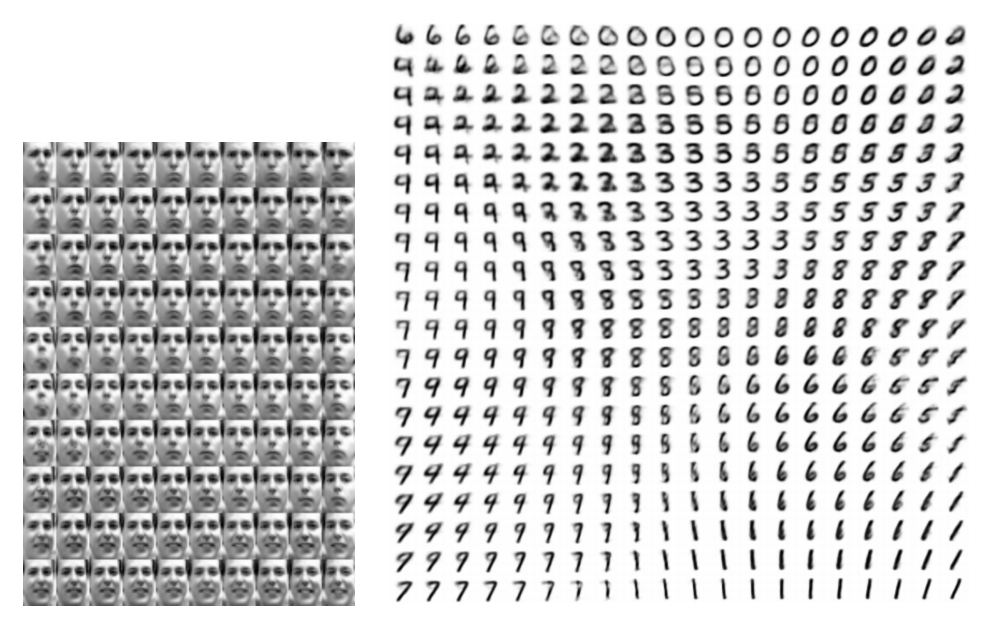
\includegraphics[width=\linewidth]{./figures/vae.png}
    \caption{VAEを用いて生成された画像の例(\cite{vae}より引用)}
    \label{fig:vae_example}
  \end{center}
\end{figure}

\section{深層状態空間モデル(DSSM)}
\label{section:dssm}

深層状態空間モデル(DSSM, Deep Karman Filters, Deep Markov Modelなどとも呼ばれる)は、VAEがデータ一つ一つの潜在表現を考えるのに対し、DSSMは時間変化があるデータの各時刻の状態表現が遷移すると考えたモデルであり、VAEを時系列方向に拡張したモデルとみなすこともできる.

深層強化学習の分野では、エージェントが環境に行動を起こした結果に観測が得られるようなときに、行動と環境の変化をモデル化する際に用いられる.本論文では一般的な以下のようなグラフィカルモデルで表されるDSSMのモデルを考えるが、行動が与えられない場合や、強化学習のように環境の状態に応じて報酬が与えられる問題に置いても以下の説明は同様にして考えることができる
.
DSSMではVAEと同じように,以下の変分下限から最尤推定によって$p(o|a)$や$p(s|x)$を得る.

\begin{eqnarray}
  \log p(o_{1:T}|a_{1:T})
  &=& \log \prod_{t=1}^T p(o_t|a_{1:t}) \nonumber \\
  &=& \log \prod_{t=1}^T \int p(o_t|s_t) p(s_t|s_{t-1}, a_t)ds_t \nonumber \\
  &=& \sum_{t=1}^T \log \int p(o_t|s_t) p(s_t|s_{t-1}, a_t)ds_t \nonumber \\
  &=& \sum_{t=1}^T \log \int q(s_t|s_{t-1}, a_t, o_t) \frac{p(o_t|s_t) p(s_t|s_{t-1}, a_t)}{q(s_t|s_{t-1}, a_t, o_t)}ds_t \nonumber \\
  &\geq& \sum_{t=1}^T \int q(s_t|s_{t-1}, a_t, o_t) \log \frac{p(o_t|s_t) p(s_t|s_{t-1}, a_t)}{q(s_t|s_{t-1}, a_t, o_t)}ds_t \nonumber \\
  &=& \sum_{t=1}^T \left( \int q(s_t|s_{t-1}, a_t, o_t) \log p(o_t|s_t)ds_t \right. \nonumber \\
  && \hspace{2em} \left. - \int q(s_t|s_{t-1}, a_t, o_t) \log \frac{p(s_t|s_{t-1}, a_t)}{q(s_t|s_{t-1}, a_t, o_t)}ds_t \right) \nonumber \\
  &=& \sum_{t=1}^T \left( \mathbb{E}_{s_t \sim q(s_t|s_{t-1}, a_t, o_t)} [\log p(o_t|s_t)] \right. \nonumber \\
  && \hspace{2em} \left. - \mathbb{E}_{s_{t-1} \sim q(s_{t-1}|s_{t-2}, a_{t-1}, o_{t-1})} [\mathrm{D_{KL}}(q(s_t|s_{t-1}, a_t, o_t) \| p(s_t|s_{t-1}, a_t, o_t))] \right)  \nonumber \\
  \label{eq:dssm_elbo}
\end{eqnarray}

ただし$s_0$は、初期状態が一定な問題を考える際は常にゼロベクトルなど一定の値にすることもあるが,そうでない場合は何らかの方法で推論する必要がある.本研究では慣例に習って$s_0$を$s_0 \sim q(s_0|\vec{0}, \vec{0}, o_0) $によって定め,(\ref{eq:dssm_elbo})の第2項の$s_0$のサンプリングはこれで置き換える.

式は、イェンセンの不等式を使い、qはpの近似である.

以上がDSSMの概要である.DSSMを用いると, \ref{fig:dssm_planet}, \ref{fig:dssm_dkf}のような新たなデータを生成することができる.actionとして回転情報が入れられている.

\begin{figure}[tbp]
  \begin{center}
    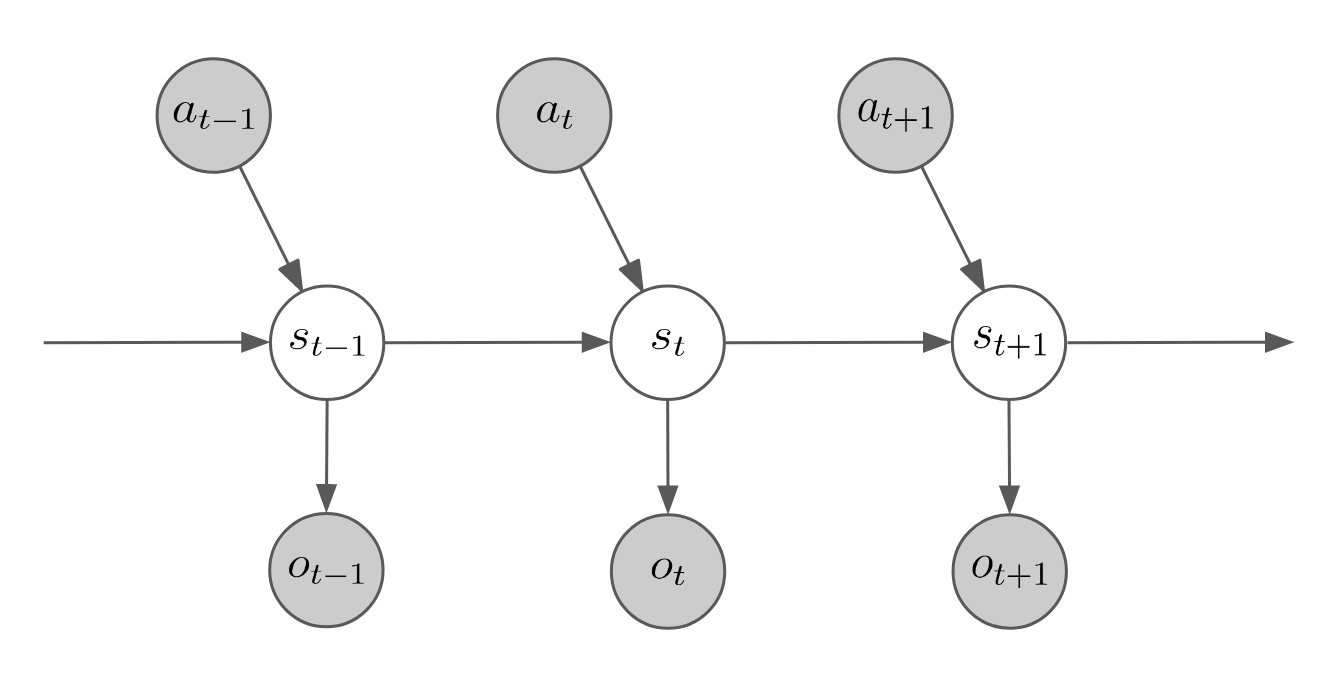
\includegraphics[width=\linewidth]{./figures/dssm.png}
    \caption{SSMのグラフィカルモデル}
    \label{fig:ssm}
  \end{center}
\end{figure}

% \caption[hoge]{fuga}
\begin{figure}[tbp]
  \begin{center}
    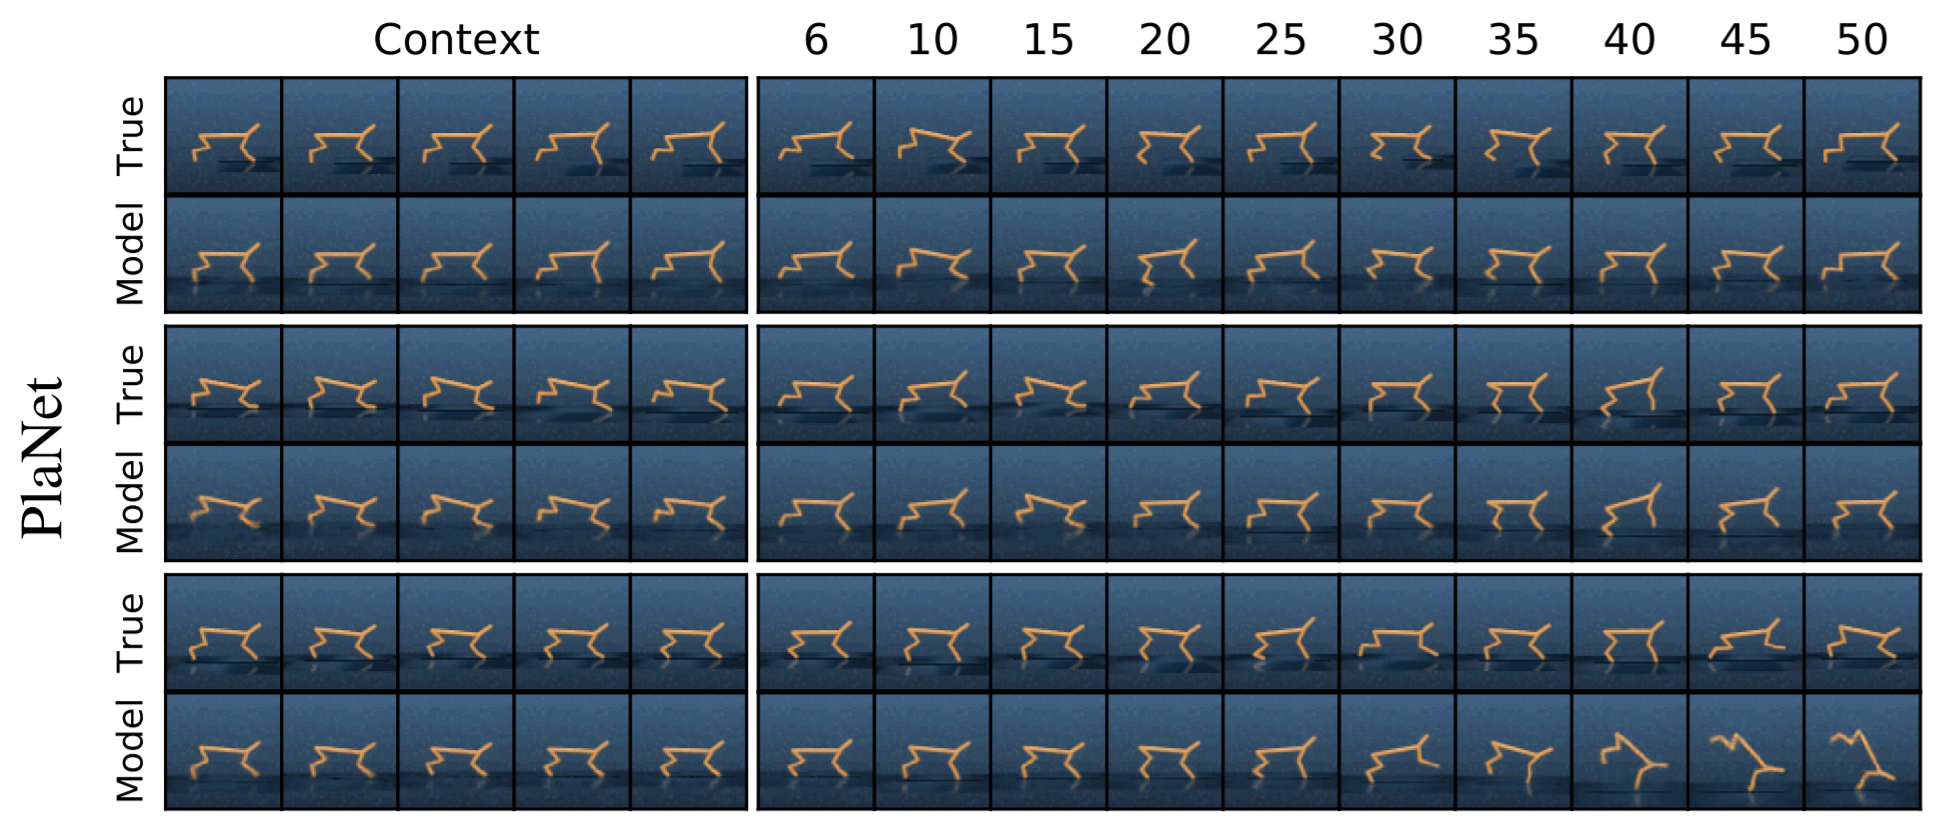
\includegraphics[width=\linewidth]{./figures/dssm_planet.png}
    \caption{DSSMで生成される映像の例.ただしSSMを少し拡張したRSSMモデルを使っている}
    \label{fig:dssm_planet}
  \end{center}
\end{figure}

% \caption[hoge]{fuga}
\begin{figure}[tbp]
  \begin{center}
    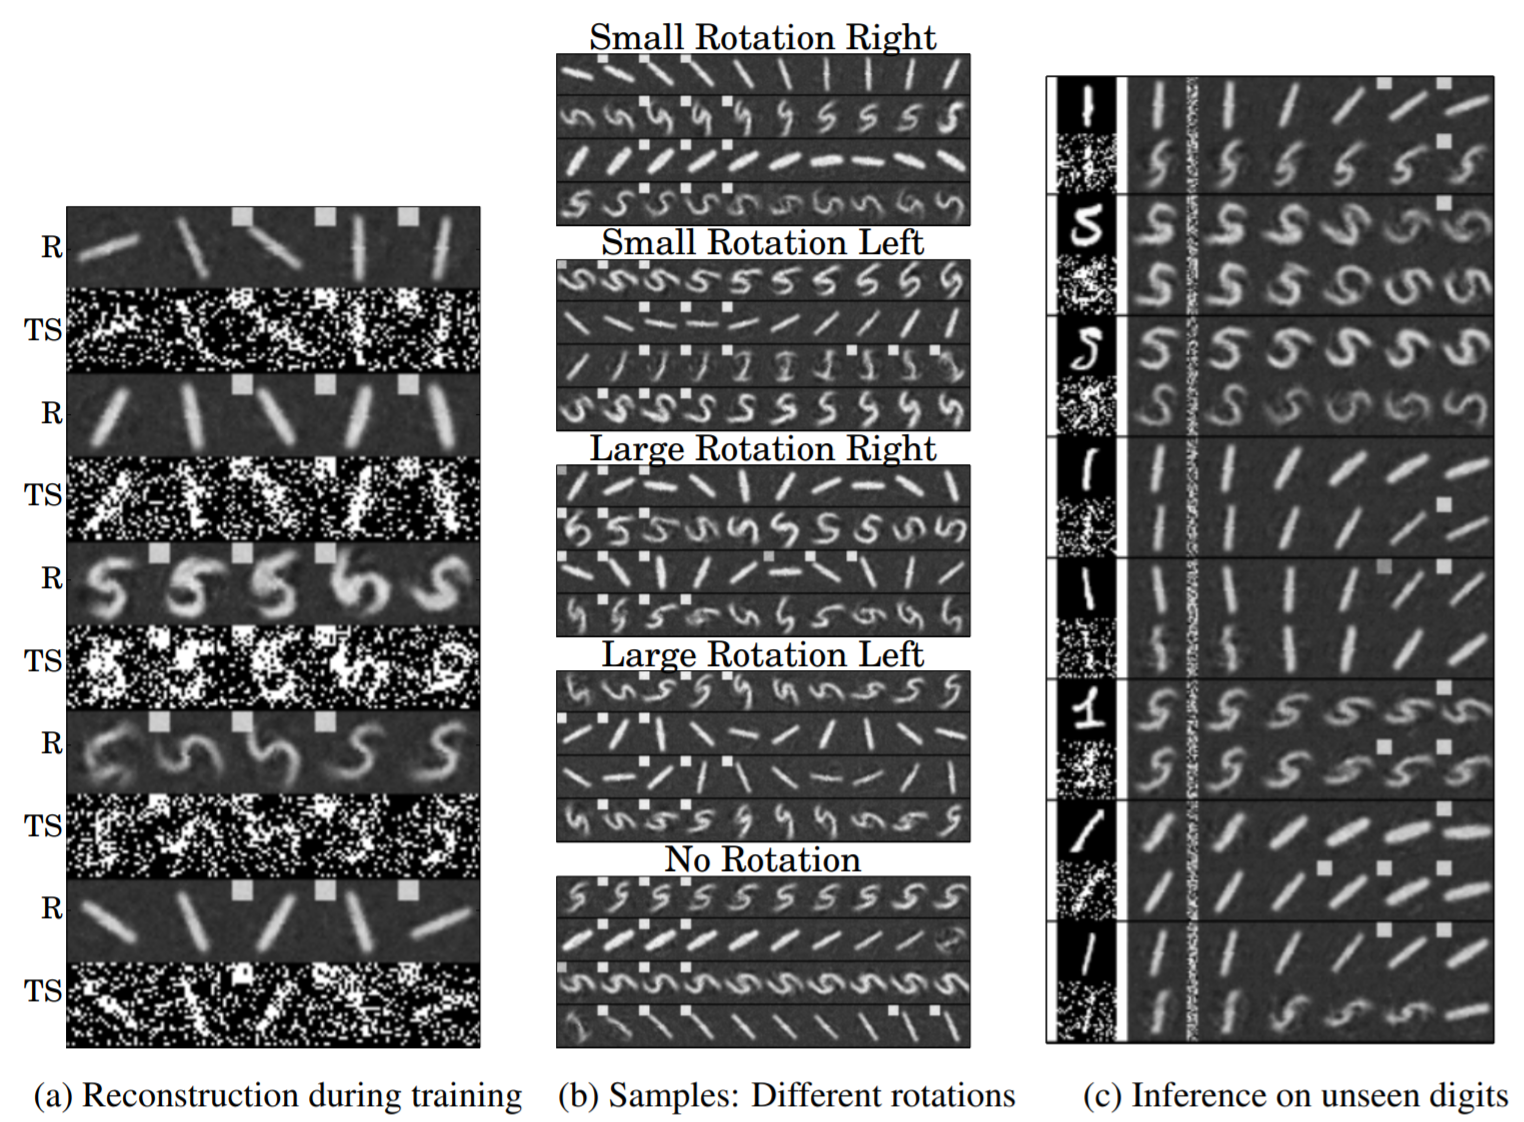
\includegraphics[width=\linewidth]{./figures/dssm_dkf.png}
    \caption{DSSMで生成される映像の例.}
    \label{fig:dssm_dkf}
  \end{center}
\end{figure}
\chapter{深層状態空間モデルの限界}
\label{chap:baseline}


深層状態空間モデルは,潜在変数の次元を大きくしたときの学習が難しい.そのことを実験的に示した上で,理論的な問題点を述べる.

\section{学習が失敗した例}
\ref{fig:dssm_failure}は,本論文の4章以降でベースラインとして述べる通常のSSMモデルを,潜在変数の次元を何通りかに変えてモデルを構築し,学習中の様子ある.潜在変数を低次元にすると順調に学習が進み,少しずつ近い映像が出力されるようになるが,次元を大きくすると途中で目的関数とする変分下限の値が正の方向に発散しやすくなる.さらに調べると,変分下限の2つの項のうち,KLダイバージェンスが先に発散していることがわかる.

% \caption[hoge]{fuga}
\begin{figure}[tbp]
    \begin{center}
      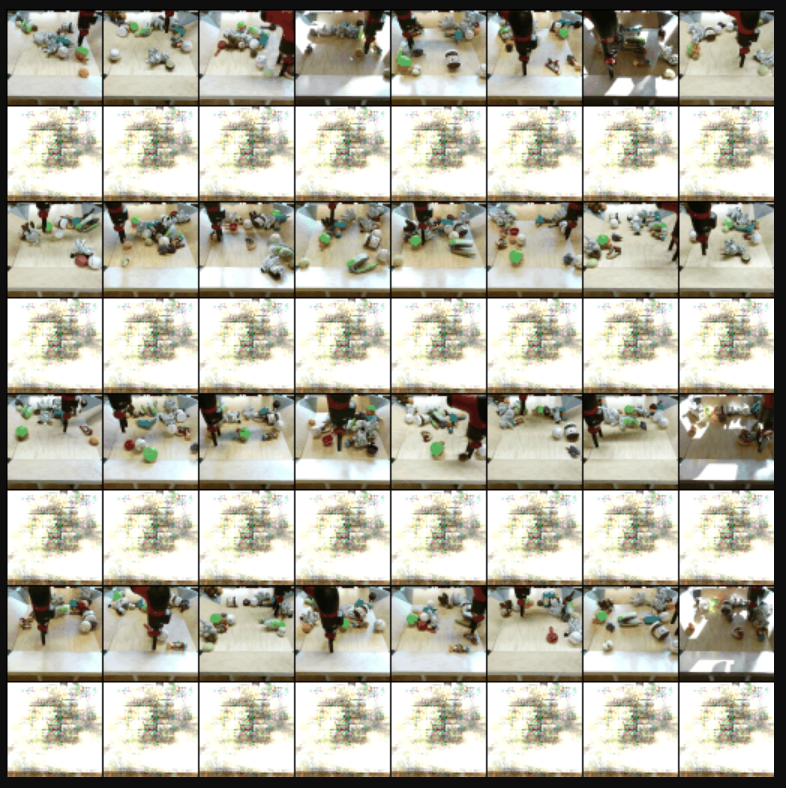
\includegraphics[width=\linewidth]{./figures/dssm_failure.png}
      \caption{DSSMの学習が失敗した例}
      \label{fig:dssm_failure}
    \end{center}
  \end{figure}

\section{深層状態空間モデルの問題点}
\begin{eqnarray}
  \end{eqnarray}
  
\begin{eqnarray}
    (VAEのELBO) \nonumber = \mathbb{E}_{\bm{z} \sim q(\bm{z}|\bm{x})} [\log p(\bm{x}|\bm{z})] - \mathrm{D_{KL}}(q(\bm{z}|\bm{x}) \| p(\bm{z})) \label{eq:vae_elbo2} \\
\end{eqnarray}
\begin{eqnarray}
    \ (DSSMのELBO) \nonumber \\
    &=& \sum_{t=1}^T \left( \mathbb{E}_{s_t \sim q(s_t|a_{1:t}, o_{1:t})} [\log p(o_t|s_t)] \right. \nonumber \\
    && \hspace{2em} \left. - \mathbb{E}_{s_{t-1} \sim q(s_{t-1}|a_{1:t-1}, o_{1:t-1})} [\mathrm{D_{KL}}(q(s_t|s_{t-1}, a_t, o_t) \| p(s_t|s_{t-1}, a_t, o_t))] \right)  \nonumber \\
    \label{eq:dssm_elbo2}
  \end{eqnarray}

VAEではこのような問題は起きない.
DSSMで学習が難しい理由として,以下が考えられる
1VAEと違い,DSSMではKL項でpriorを近づけ先であるposteriorが固定されていない.
2stateの次元が小さく,$H(o) >> H(s_{prev})$ であるときのposteriorの出力は一意に定まり
stateの次元が大きく $H(o) >> H(s_{prev})$でない時は安定しない
近似がゆるくなる!!!!!
また,stateの推論にモンテカルロ近似をするが,その時のサンプル回数Lを増やすて平均を取ることは,経験的にうまく行かないことが知られてたりするのかな…?

近づけ先が固定されていないときにKLがnanすることは,Variational Autoencoder with Arbitrary Conditioningなどでも言われている

\chapter{状態表現の階層性を考慮することによる深層状態空間モデルの拡張}
\label{chap:proposal}

第三章の問題を受け,第四章ではシンプルな帰納バイアスを導入することによってDSSMを拡張する方法を提案する.はじめに本研究で扱う問題設定について改めて整理し,続けて提案手法とその既存の類似手法について述べる.

\section{問題設定の整理}

本研究では行動条件付き映像予測の問題を解く.具体的には,ある行動主体が実行した行動系列$a_{1:10}$と初期観測$o_0$が与えられたときに$o_{1:10}$を生成し,その生成される映像の尤度を高めることを目指す.ただし訓練時には行動系列と観測系列の組$\{\vec{a}, \vec{o}\}$の訓練用のデータセットを用いることができ,評価時には,訓練データには含まれないが訓練データと同じ条件で収集された評価用のデータセットを用いる.
本研究の目的は,この条件付き映像予測問題においてベースラインにDSSMを設定し,DSSMをより複雑な環境での映像予測問題にもスケールできるように拡張することである.

\section{提案手法}
三章で述べたようにベースラインのDSSMでは潜在変数の次元を大きくすると学習がうまくいかなかった.しかし予備実験で得た,低次元の潜在変数を用いたときには部分的に学習が進んだという事実をヒントにし,状態変数の次元を大きくしていく方向性はそのままで状態表現の階層性を考えることにより,より複雑な問題設定においても学習可能なDSSMの拡張方法を提案する.

\begin{figure}[tp]
  \begin{center}
    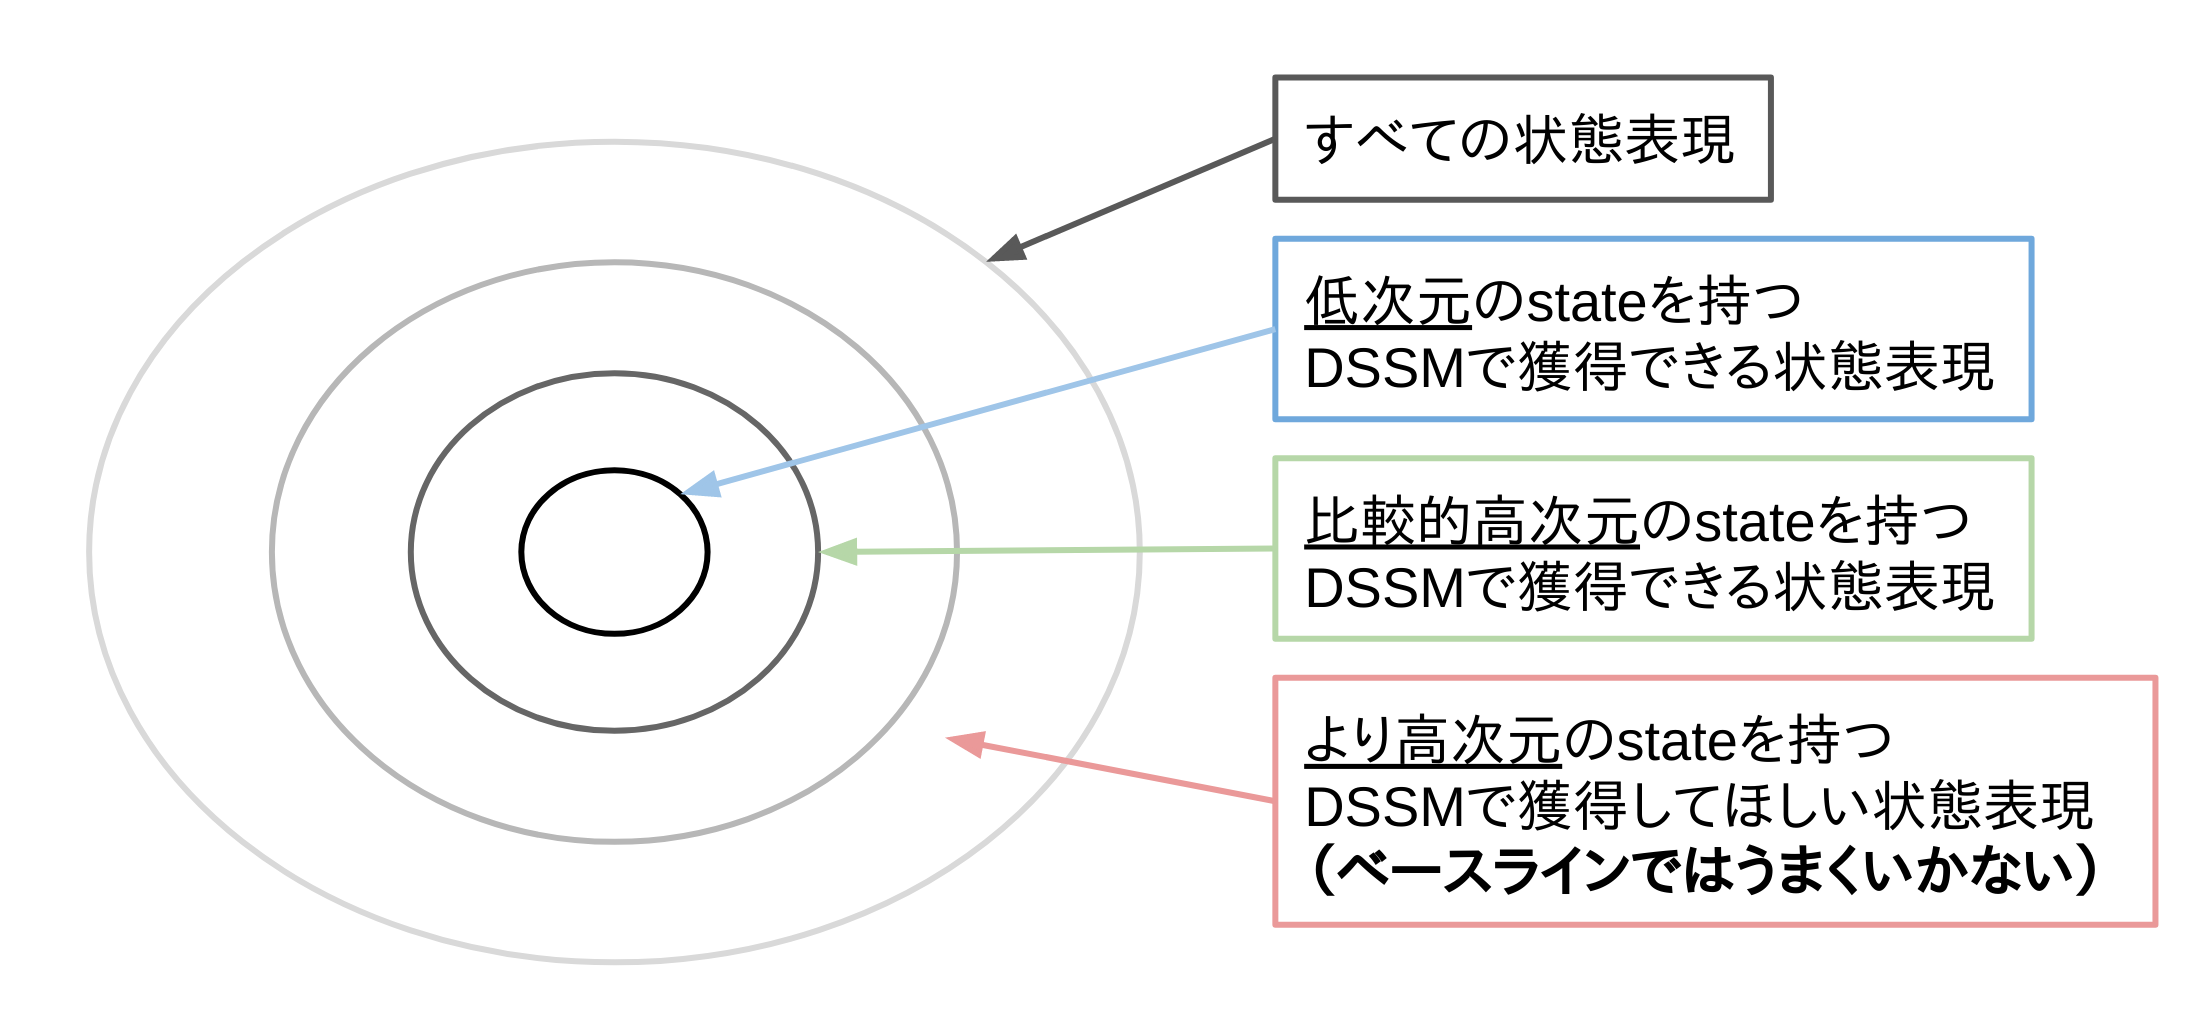
\includegraphics[width=\linewidth]{./figures/hierarchical.png}
    \caption{hierarchical}
    \label{fig:hierarchical}
  \end{center}
\end{figure}

\subsection{状態表現の階層性}
はじめに,ベースラインのDSSMにおいて潜在変数の次元を変えた時に獲得される情報について考察する.低次元の状態変数で獲得できる情報は高次元の状態変数を用いた場合にも当然獲得できると考えた場合,図(\ref{fig:hierarchical})のように高次元の状態変数が持つ情報は低次元の状態変数が持つ情報をほぼ内包していると考えることができる.
ここで状態変数の次元をより大きくしたときに精度がむしろ悪化することが問題であったが,これは三章で述べたとおり,状態変数の次元が大きくなったときに高次元ベクトルから高次元ベクトルへの写像を学習する必要が生じあるべき写像先がなかなか定まらないことが原因であると考えられ,何らかの方法で遷移モデルの学習を補助することで図のようにより多くの情報を獲得できる可能性がある.

\subsection{階層的な状態表現の遷移}
ベースラインの状態表現の遷移は図(\ref{fig:transition_base})が示すように状態変数が持つすべての情報を一度に変換することを考えているが,直感的に一括で変換することは学習が難しいと思われる.状態表現を一括で変換する代わりに,前節のような階層性の概念を導入することで図(\ref{fig:transition_proposal})のように簡単に遷移が学習できる部分から順に遷移させていくような方法を考えることができる.

このような階層的な状態表現の遷移を考えると,はじめから高次元の状態表現の遷移を考えずに学習の習熟度に合わせて徐々に高次元の状態ベクトルの遷移を学習することができ,学習がスムースに進みやすくなると考えられる.

\begin{figure}[tbp]
  \begin{center}
    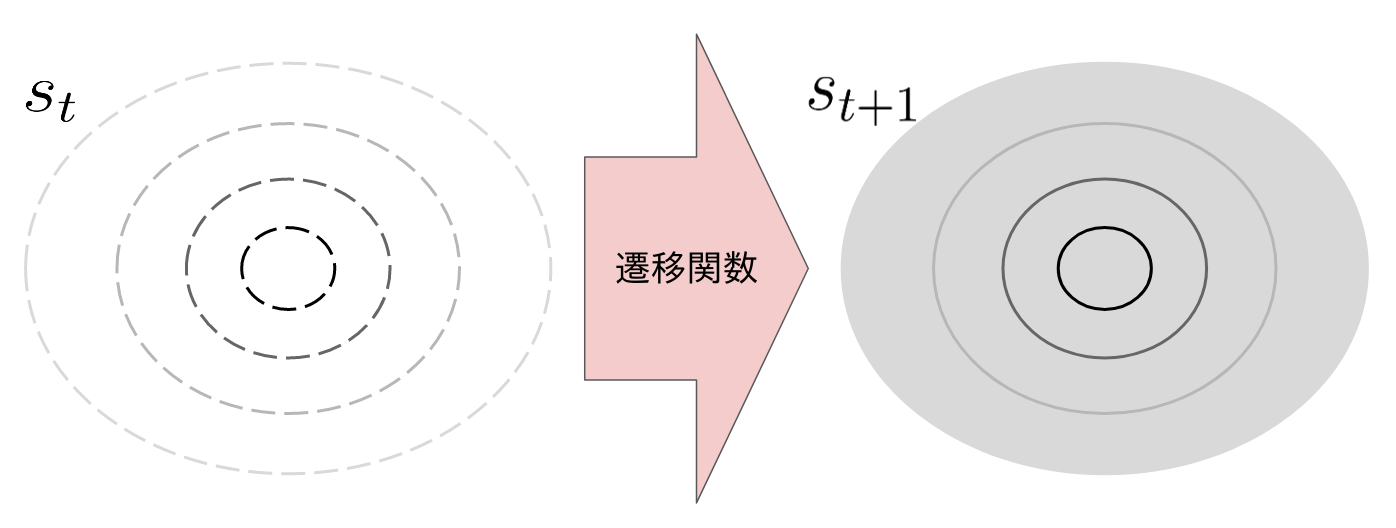
\includegraphics[width=0.5\linewidth]{./figures/transition_base.png}
    \caption{transition base}
    \label{fig:transition_base}
  \end{center}
\end{figure}

\begin{figure}[tbp]
  \begin{center}
    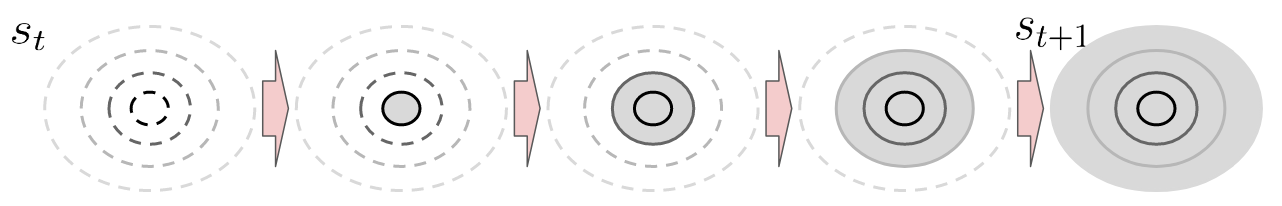
\includegraphics[width=0.8\linewidth]{./figures/transition_proposal.png}
    \caption{transition proposal}
    \label{fig:transition_proposal}
  \end{center}
\end{figure}

% \caption[hoge]{fuga}
\begin{figure}[tbp]
  \begin{center}
    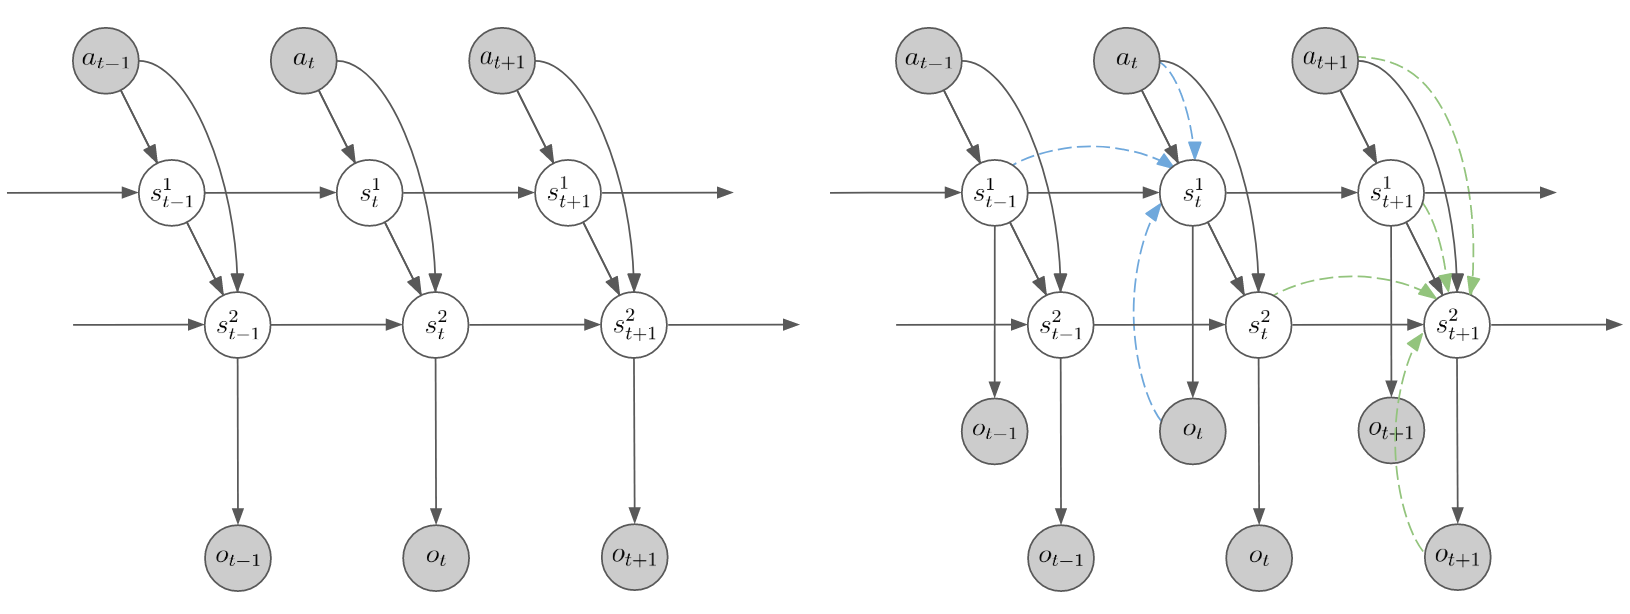
\includegraphics[width=\linewidth]{./figures/proposal.png}
    \caption[提案手法のグラフィカルモデル]{提案手法のグラフィカルモデル.点線の$s^1$, $s^2$の推論分布は簡単のため時刻t, t-1でのみ記載している.proposal (学習時) 2つずつ記載されている$o_t$は同じデータを示すが.異なるsから独立に生成されることを明示している.}
    \label{fig:proposal}
  \end{center}
\end{figure}

\subsection{確率モデル・最適化}

ここまでで状態変数の階層性とその遷移を考えたが,この階層性の仮定はDSSMの性能の向上に十分寄与しうると考え,状態変数の階層性を帰納バイアスとしてDSSMに組み込み以下のようなモデルとその最適化アルゴリズムを提案する.

\vspace{\baselineskip}
提案手法のグラフィカルモデルを図(\ref{fig:proposal})に示す.(TODO: 三層以上の場合も図にする),
提案手法は,DSSMの状態変数をN層に階層化したモデルである.図(\ref{fig:proposal})は2階層の提案モデルを図(\ref{fig:proposal_big} TODO)は3階層以上の提案モデルを表している.図(\ref{fig:proposal})の上側の状態変数から一階層の状態変数・二階層の状態変数と呼ぶことにすると一階層の状態変数が低次元ベクトル,二階層の状態変数が高次元ベクトルになっており,高次元の状態変数の生成・推論時に低次元の状態変数を用いるようなモデルになっている.高次元の状態変数の遷移時に低階層の状態変数を用いて写像先に関する情報を補助的に与えることで,学習を安定化させる効果が期待される.またモデルの評価時には,最高層の観測の生成モデル $p(o_t|s^N_t)$ を用いる.

\begin{algorithm}[tbp]               
  \caption{N階層DSSMの学習アルゴリズム TODO: 書き直す}
  \label{alg1}                          
  \begin{algorithmic}
    \FOR{一階層目からN階層目まで}
      \WHILE{学習が収束していない}
        \STATE 現在の階層より上の階層のパラメータを固定し, 
        \STATE 現在の階層を以下の目的関数で学習する
        \STATE $L(x)$ = その階層での再構成 + その階層の$KL(q||p)$ \\
      \ENDWHILE
    \ENDFOR
  \end{algorithmic}
\end{algorithm}

\vspace{\baselineskip}
次に提案手法の学習アルゴリズムをアルゴリズム\ref{alg1}に示す.この学習アルゴリズムは前節「階層的な状態表現の遷移」で述べた,習熟度に合わせて徐々に高次元の状態ベクトルの遷移を学習するという考え方に基づいており,これにより安定した学習が見込める.今回簡単のために高階層の潜在表現の学習時にはそれより低階層の状態表現の学習を止めているが,他の方法も考えられ,これついては考察「低次元状態ベクトルの階層の再学習」で述べる.



% 確率的生成過程は以下
% \begin{equation}
%   p(o_{1:T}|a_{1:T}) = \prod_{t=1}^T \iint p(o_t|s^2_t) p(s^2_t|s^2_{t-1}, a_t, s^1_t) p(s^1_t|s^1_{t-1}, a_t) d{s^1_t}{ds^2_t}
% \end{equation}


% この時の変分下限は以下
% \begin{eqnarray}
%   \ (ELBO) \nonumber \\
%   &=& \sum_{t=1}^T \left( \mathbb{E}_{s^2_t \sim q(s^2_t|a_{1:t}, o_{1:t})} [\log p(o_t|s^2_t)] \right. \nonumber \\
%   && \hspace{2em} \left. - \mathbb{E}_{s^1_{t-1} \sim q(s^1_{t-1}|a_{1:t-1}, o_{1:t-1}), 改行したい s^2 \sim}  [\mathrm{D_{KL}}(q(s_t|s_{t-1}, a_t, o_t) \| p(s_t|s_{t-1}, a_t, o_t))] \right. \nonumber \\
%   && \hspace{2em} \left. - \mathbb{E}_{s^1_{t-1} \sim q(s^1_{t-1}|a_{1:t-1}, o_{1:t-1}), 改行したい s^2 \sim } [\mathrm{D_{KL}}(q(s_t|s_{t-1}, a_t, o_t) \| p(s_t|s_{t-1}, a_t, o_t))] \right) \nonumber \\
%   \label{eq:hssm_elbo}
% \end{eqnarray}


% 目的関数は以下
% % 
% \begin{eqnarray}
%   \ (目的関数) \nonumber \\
%   &=& \sum_{t=1}^T \left( \mathbb{E}_{s^2_t \sim q(s^2_t|a_{1:t}, o_{1:t})} [\log p(o_t|s^2_t)] + \beta \mathbb{E}_{s^1_t \sim q(s^1_t|a_{1:t}, o_{1:t})} [\log p(o_t|s^1_t)] \right. \nonumber \\
%   && \hspace{2em} \left. - \mathbb{E}_{s^1_{t-1} \sim q(s^1_{t-1}|a_{1:t-1}, o_{1:t-1}), 改行したい s^2 \sim}  [\mathrm{D_{KL}}(q(s_t|s_{t-1}, a_t, o_t) \| p(s_t|s_{t-1}, a_t, o_t))] \right. \nonumber \\
%   && \hspace{2em} \left. - \mathbb{E}_{s^1_{t-1} \sim q(s^1_{t-1}|a_{1:t-1}, o_{1:t-1}), 改行したい s^2 \sim } [\mathrm{D_{KL}}(q(s_t|s_{t-1}, a_t, o_t) \| p(s_t|s_{t-1}, a_t, o_t))] \right) \nonumber \\
%   \label{eq:hssm_loss}
% \end{eqnarray}

\section{類似手法との差分 TODO}
提案手法と類似手法の差分について整理する.DSSM自体を用いた映像予測の研究はこれまであまりされていないが,これは1章でも述べたとおりDSSMは自己回帰モデルと比べて高精度な生成には向いていないためだと考えられる.そのため本節では階層性を考慮した画像生成と映像生成の既存研究について取り上げる.

まずモデルに階層性を取り入れた画像生成の先行研究としてDRAW[引用],PGGAN[引用]があり,映像予測で階層的なモデルを扱う手法としFutureGAN[引用],てVRNN[引用]がある.DRAWはVAEベースの深層生成モデルであり,潜在変数を複数用意し階層的にすることでデータの潜在表現に単純な正規分布を仮定しないより複雑な表現を可能にしている.提案手法はDRAWを時間変化するデータを扱う問題設定に拡張したようなモデルとなっているが,DRAWは一度にすべての潜在表現を学習するのに対し,時系列データを扱う提案手法では毎時刻の状態表現の遷移を学習することが難しいため潜在表現を順に学習するアルゴリズムを採用している.PGGANは敵対的生成モデルを用いた画像生成手法で,低解像度の画像の生成からはじめ,学習が進むにつれてニューラルネットワークモデルを徐々に多層にすることで高解像度の画像生成を行う.低次元の隠れ変数を変数から学習していくという点で提案手法と似ているが,PGGANは何も条件付けしない生成を行っており,過去の状態や行動で条件付けして画像を生成する行動条件付き映像予測の問題設定に用いる方法は自明ではなかった.FutureGANはPGGANを映像予測に応用した手法で,過去の6フレーム程度の映像を入力とし未来の25フレーム程度の映像を予測することができる.VRNNは直前のフレームを用いて次のフレームを予測する自己回帰モデルになっており,潜在変数から画像を出力する過程で得られる隠れ変数を次の時刻の画像の出力にも用いるようにして潜在変数の階層性を考えたモデルになっている.FutureGANやVRNNは予測する際に過去数フレームの映像を用意する必要があるが,ベースラインのDSSMや提案手法では初期状態の推論用に過去1フレームだけを用いれば良いモデルになっている.

RNNやLSTMを用いた自己回帰モデルになっており,
\begin{itemize}
  \item DRAW[]はVAEの潜在変数に階層性をもたせたモデル画像生成で用いられる
  \item 多層RNN[]は
  \item PGANは平面状の隠れ変数の次元を徐々に大きくすることで徐々に高解像度の映像生成を可能にする敵対的生成ネットワークベース手法で,
  \item FutureGANは,6フレームの映像を入力としてその後に続く30フレームを予測するような問題設定を解くGANベースの手法で,潜在変数を徐々にある.こちらは入力として複数フレーム与えられるので本研究の
  また,確率的な遷移を考えていない.
\end{itemize}

表:必要な入力フレーム数,条件付け,映像か画像か

% あれaction conditionlな先行研究って,visual forsightとか,SV2Pとかしかなかったっけ?

% videoflowはaction conditionalじゃないしー


\chapter{実験}
\label{chap:experiment}
第4章で述べた提案手法の有効性を検証するために,BAIR Push Datasetという行動条件付き映像予測用のデータセットを用いて評価実験を行った.本章では実験の内容について説明した後に実験結果について述べる.

\section{実験内容}
第4章で述べた提案手法とベースラインの比較を行う.ベースラインは第二章で述べたシンプルなDSSMとし,状態ベクトルの次元を64, 256, 512, 1024の4通りに変えて実験を行う.提案手法は64次元と512次元の二階層の状態ベクトルを持つモデルと,64次元と512次元と1024次元(TODO うまく行けば)の三階層の状態ベクトルを持つモデルとした.ベースラインと提案手法の実装の差は必要最小限にとどめ,どちらも学習時には10フレーム先までの予測を行った.またパラメータの最適化にはそれぞれ確率的勾配降下法アルゴリズム Adam[引用] を用いた.
評価指標には,定量評価として予測誤差(負の対数尤度)を測り,合わせて定性評価も行う.またこれらの評価時には,DSSMと同じデコーダー・エンコーダーモデルを持つVAEを用意し,時系列方向の遷移を学習する必要がない場合の生成モデルの精度とも比較を行う.(この実験自体TODO.)

\subsection{データセット}
(TODO: データセットを紹介する図を入れる)

今回用いるBAIR Push Datasetは行動条件付き映像予測と行動条件をつけない映像予測のどちらの研究でも用いられるデータセットであり,カリフォルニア大学バークレー校によって制作・公開されている.[引用]
こちらのデータセットは,様々な物体がおかれた机の上をロボットアームがランダムに掻き乱すようにして様々なデータが記録されており,今回はその中から行動系列$\vec{a}$と固定視点から観測された画像系列$\vec{o}$を用いる.今回用いる行動系列$\vec{a}$は,具体的にはロボットのエンドエフェクタの位置姿勢の命令値になっている.観測画像は64x64サイズのRGB画像で,これらのデータは10hzで撮られている.また訓練時と評価時に使われる物体は揃えられている.

\subsection{ベースラインの実装}
実装にはFacebook社製の深層学習フレームワークであるPytorch[引用]と,松尾研究室研究員の鈴木さんが中心となって開発されている深層生成モデルライブラリPixyz[引用]を主に用いた.学習用データの読み込みとその最適化にはGoogle社製の深層学習フレームワークであるTensorFlow[引用]を用いた.また実装では,DSSMを用いた強化学習手法であるPlaNetの公開実装[引用]を参考にした.
まずベースラインの実装を説明した後,提案手法の実装について述べる.

\subsubsection{モデルアーキテクチャ}
ベースラインは4つの部分モデルから構成される.
\begin{itemize}
    \item デコーダー $p(s_t|x_t)$
    \item エンコーダー $q(x_t|h_t)$
    \item 遷移モデル(事前分布) $p(s_t|s_t-1, a_t)$
    \item 遷移モデル(事後分布) $q(s_t|s_t-1, a_t, h_t)$
\end{itemize}

遷移モデル(事前分布)とデコーダーが生成モデルに相当し,提案手法のグラフィカルモデルの実践部分を表しす.遷移モデル(事後分布)とエンコーダーが推論モデルに相当し,提案手法のグラフィカルモデルの点線部分を表している.

\begin{description}
    \item[デコーダー・エンコーダー]\mbox{}\\
(図TODO)
PlaNetに倣い,デコーダー/エンコーダーモデルにはWorldModel(Ha 2018)の論文中に記載されているモデルを採用した.デコーダーは各時刻の状態ベクト$s_t$を全結合層で1024次元の隠れ変数に変換したあと,4層の逆畳み込み層で観測画像と同じサイズである64x64サイズのRGB画像に変換する.出力は各ピクセルごとに正規分布をおくが,本研究では簡単のためその分散はそれぞれ1に固定している.
エンコーダーは各時刻の観測を4層の畳み込み層と1層の全結合層で1024次元の隠れ変数$h_t$に変換する.

本研究では,状態変数の次元を変えた際にも隠れ層のパラメータ数などは一切変えなかった.

    \item[遷移モデル]\mbox{}\\
(図TODO)
遷移モデルには,ある時刻の状態ベクトル$s_t$を生成過程に従って生成する事前分布モデルと,ある時刻の観測$o_t$も与えられたときに$s_t$を推論する事後分布モデルの2種類を用意する.

この2つのモデルはアーキテクチャはほとんど共通で入力とするデータだけが違い,事前分布モデルでは一つ前の時刻の状態$s_{t-1}$と行動$a_t$を入力とするが事後分布ではそれに加えその時刻の観測$o_t$をエンコードして得たデータ$h_t$を入力とする.出力はどちらのモデルも次の時刻の状態ベクトルの分布の母数(平均と標準偏差)である.
アーキテクチャは,入力情報をすべて連結して一度全結合層で変換したものを平均を求める全結合層と標準偏差を求める全結合層のそれぞれで変換し,求めたい分布の平均と標準偏差を出力する.

\end{description}

\subsubsection{学習の安定化}
潜在変数の次元を大きくした際,学習の初期段階でカルバックライブラー距離の計算値が発散することがよく起こる.これは遷移モデルが次の時刻の状態ベクトルの分布の標準偏差として0に非常に近い値を出力してしまった結果(丸め誤差が発生して)カルバックライブラー距離の計算時にゼロ除算が発生してしまうためである.この問題は遷移モデルが出力する標準偏差に下限を設けることで解決することができる.今回の実験では潜在変数の次元を1024次元にした際にこのカルバックライブラー距離が学習開始後直ちに発散する問題が発生したので,標準偏差の下限値を$10^{-7}$とすることで学習をある程度継続することができた.ただし標準偏差に下限を設けることは経験的に学習を難しくすることがわかっていたので,他の条件での実験の際には適用しなかった.

\subsection{提案手法の実装}
提案手法はベースラインの節で説明した部分モデルをほぼそのまま用いる.二階層目以上の第i層では,各遷移モデルの入力として一時刻前の状態変数$s^i_{t-1}$と行動$a_t$だけでなく,一つ低次元の層の同じ時刻の状態ベクトル$s^{i-1}_t$も入力とする.また,提案手法では,パラメータを固定している層の状態ベクトルのサンプリングには,モデルの評価時の設定に合わせて常に事前分布を用いている.これは,パラメータを固定している層はそれ以上学習されないために,事前分布より良い表現が下の階層に渡されることはなく,むしろ事前分布で足りない表現を積極的に下の階層の学習で獲得できるようにするためである.
その他はベースラインの実装と変えていない.


\section{実験結果}

簡単のため,ここから状態変数の次元を64にしたベースラインモデルを「ベースライン(64)」,状態変数の次元を64と512にした提案手法モデルを「提案手法(64 + 512)」などと呼ぶ.

\subsection{定量評価(尤度)}

\begin{figure}[tp]
    \begin{center}
        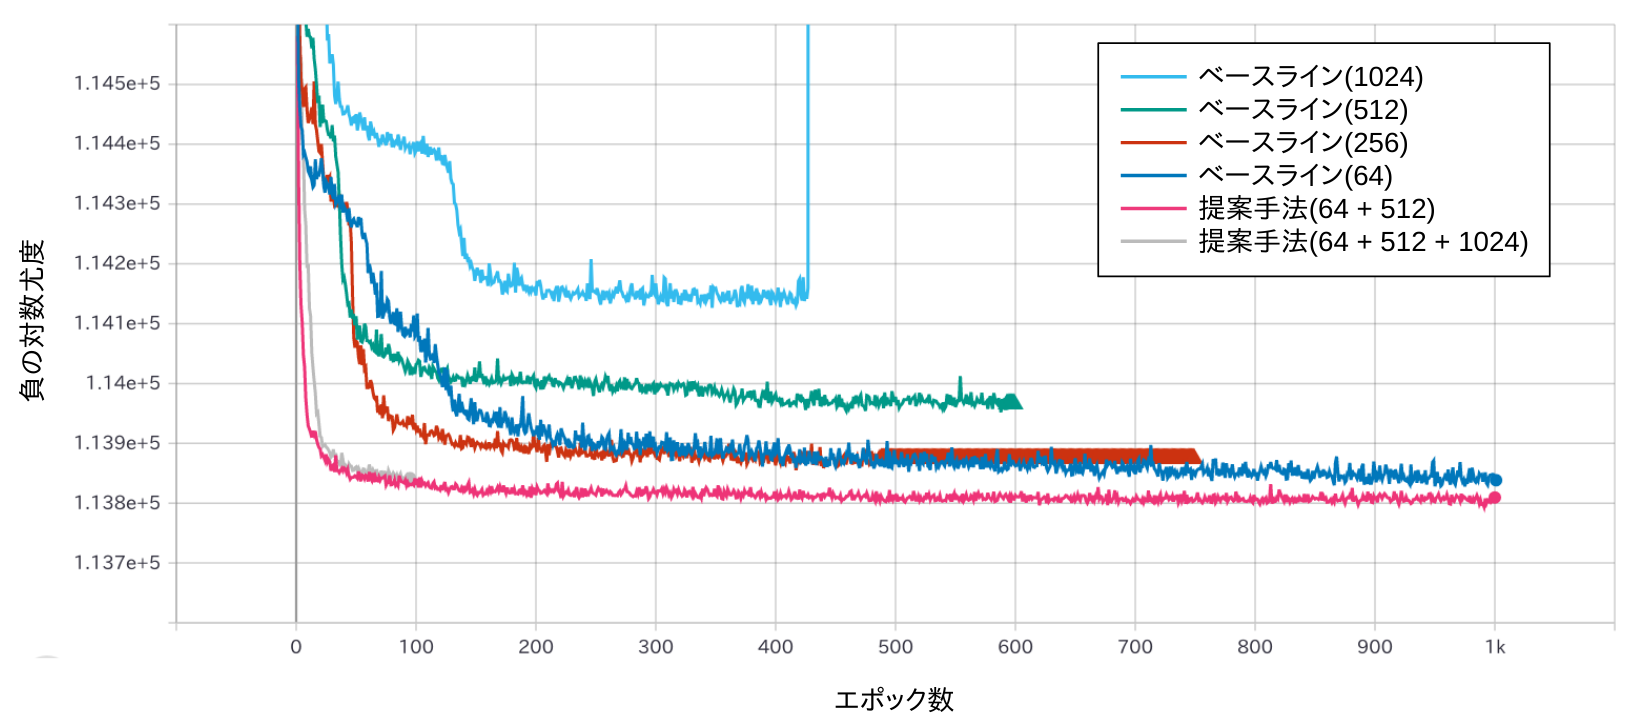
\includegraphics[width=\linewidth]{./figures/curve.png}
        \caption[提案手法の学習曲線]{提案手法の学習曲線 一番下が提案手法.TODO: 綺麗にする}
        \label{fig:curve}
    \end{center}
    \end{figure}

\begin{table}[tbp]
    \begin{center}
    \caption{手法ごとの定量評価指標(尤度)}
    \begin{tabular}{|c||c|} \hline
      手法 & 負の対数尤度 \\ \hline \hline
      ベースライン(64) & $1.1384 \times 10^5 $ \\ \hline
      ベースライン(512) & $1.1397 \times 10^5 $ \\ \hline
      ベースライン(1024) & $1.1416 \times 10^5 $ \\ \hline
      提案手法(64 + 512) & $\bm{1.1381 \times 10^5 }$ \\ \hline
      提案手法(64 + 512 + 1024) & $1.1383 \times 10^5$ \\ \hline
    \end{tabular}
    \label{table:evaluation}
    \end{center}
  \end{table}
  

図(\ref{fig:curve})は,ベースラインと提案手法の学習時の評価用データでの負の対数尤度の値の推移をプロットしたもの(学習曲線)である.ただし提案手法(64 + 512)は一階層部分に1000 epoch 学習したベースライン(64)を用いており,学習曲線としてプロットされているのは二階層部分の学習時の負の対数尤度である.同様に提案手法(64 + 512 + 1024)は一階層部分に1000 epoch 学習したベースライン(64)を,二階層部分に1000 epoch 学習した提案手法(64 + 512)を用いており,学習曲線としてプロットされているのは三階層部分の学習時の負の対数尤度である.また表(\ref{table:evaluation})に最終的な負の対数尤度を示す.

まず図(\ref{fig:curve})について,ベースライン(512)と提案手法(64 + 512)との比較から,二階層にすることで潜在変数の次元を512次元と大きくした際にもうまく学習が進むようになったことがわかる.これは,高次元の状態変数の学習時に学習済みの低次元の状態変数の情報を用いることで狙い通り学習が安定したためだと考えられる.次にベースライン(64)と提案手法(64 + 512)の比較から,高次元の潜在変数で学習させたことによってより高い尤度の映像を生成できるようになったことがわかる.これは潜在変数を高次元にした方が多くの情報を保持しやすく,適切に学習が進みさえすれば予測性能が向上しやすくなるためだと考えられる.最後に三階層の提案手法(64 + 512 + 1024)について見ると,ベースライン(1024)と比較し明らかに学習が進んだものの,ベースライン(64 + 512)と比較して精度の改善は見られず,潜在変数の次元を大きくすることだけでは精度の向上には限界があるということが伺える.

\subsection{定性評価}
図(\ref{fig:compare_ab}),図(\ref{fig:compare_cd})は評価用データで10フレームの行動条件付き映像予測により生成された映像のサンプルで,正解映像とベースライン(64)による予測映像,提案手法(64 + 512)による予測映像を比較している.どちらのモデルもロボットアームの位置はほぼ正しく予測ができているが,環境中の物体の見た目には差が見られた.図(\ref{fig:pred_a}), 図(\ref{fig:pred_b})を見ると,ベースラインでは環境中の物体の輪郭がぼやけて灰色がかっているのに対し,提案手法では特に物体が密集していない場合に比較的物体一つ一つの生成が鮮明になっていることが見て取れる.これは潜在変数の次元を大きくし保持できる情報を増やすことに成功したためだと言える.しかしフレームごとの見た目には改善が見られたものの,物理的な操作についての予測はあまり改善が見られなかった.図(\ref{fig:pred_c})では,正解映像ではロボットアームの移動によって中央の緑の物体の姿勢を変えているが,そもそもベースラインではその物体を生成できておらず,提案手法でも僅かに黒っぽい点として表されている程度で姿勢の変化を読み取ることはできない.図(\ref{fig:pred_d})は,正解映像では滑らせるようにして2つの物体を近づけており,提案手法のでは2つの物体の輪郭が見られるが,机の色やロボットアームの色と途中から同化してその動きを追うことは困難である.このように物理的な操作の予測を改善するにはまず一フレーム一フレームの質を上げる必要があると考えられ,今回は物理的な操作の予測の改善はあまり見られなかった.最後に図(\ref{fig:pred_long})は,各モデルで学習時よりも長い30フレームの映像予測をした際の生成映像である.ベースライン・提案手法ともにロボットアームの動きはほぼ正解映像と一致しているが,ベースラインでは右端に映る物体が映像を予測するにつれて青色から緑色に変わってしまっているのに対し,提案手法は背景や周りの物体について一貫性が保たれていた.これは,潜在変数の次元が小さいまま性能をあげようとすると潜在表現に含まれる情報が密になりすぎて遷移時に遷移とは関係のない情報も変化させてしまいやすいという問題がある可能性があり,一方提案手法は高次元の潜在変数を使うためにそのような問題は生じなかったと考えられる.

% また図(\ref{fig:pred_a})では,水色の物体の予測位置が提案手法が生成した映像と正解映像とで少しずつずれているが,このことから画像を一画素ずつ潜在表現で記憶しているのではなく,物体の見た目と位置を別々に保存するように学習がすすんでいたことが伺える.

% 高次元で学習できるようになった.これは深層状態空間モデルの大きな問題点を克服できたと言える.

\begin{figure}[tp]
    \centering
    \subfloat[]{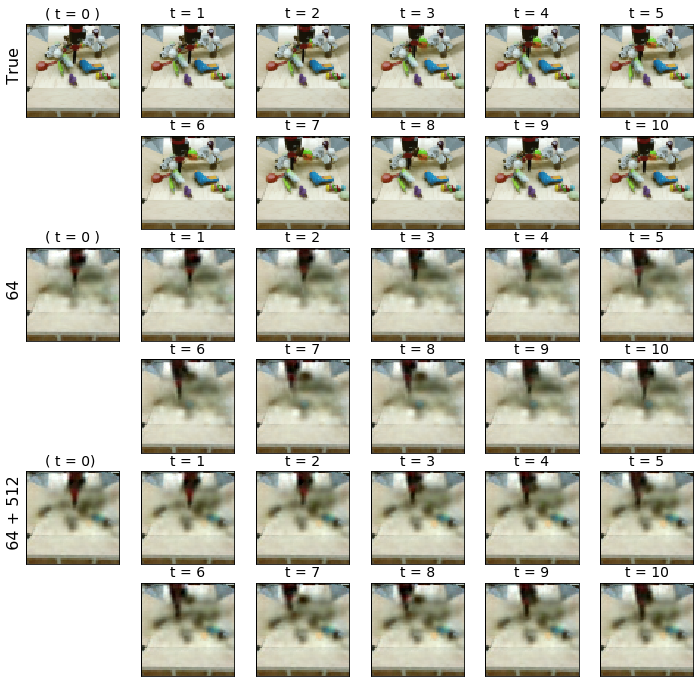
\includegraphics[clip, width=0.63\linewidth]{./figures/pred_a.png}
    \label{fig:pred_a}}
    \\
    \subfloat[]{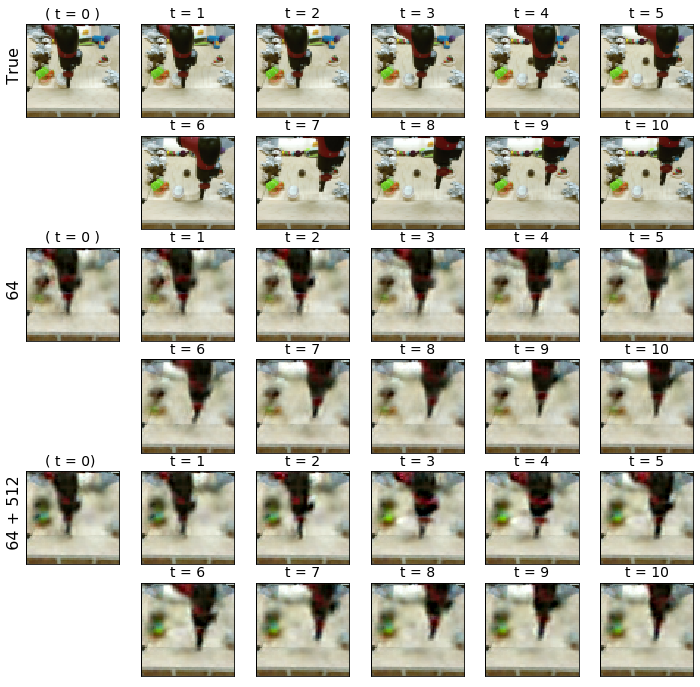
\includegraphics[clip, width=0.63\linewidth]{./figures/pred_b.png}
    \label{fig:pred_b}}
    \caption[映像予測結果1]{映像予測結果1.「True」が正解映像,「64」がベースライン(64)での予測結果,「64 + 512」が提案手法(64 + 512)での予測結果を示す.また$t = 0$は初期状態の推論時に与えられるフレーム.}
    \label{fig:compare_ab}
\end{figure}

\begin{figure}[tp]
    \centering
    \subfloat[]{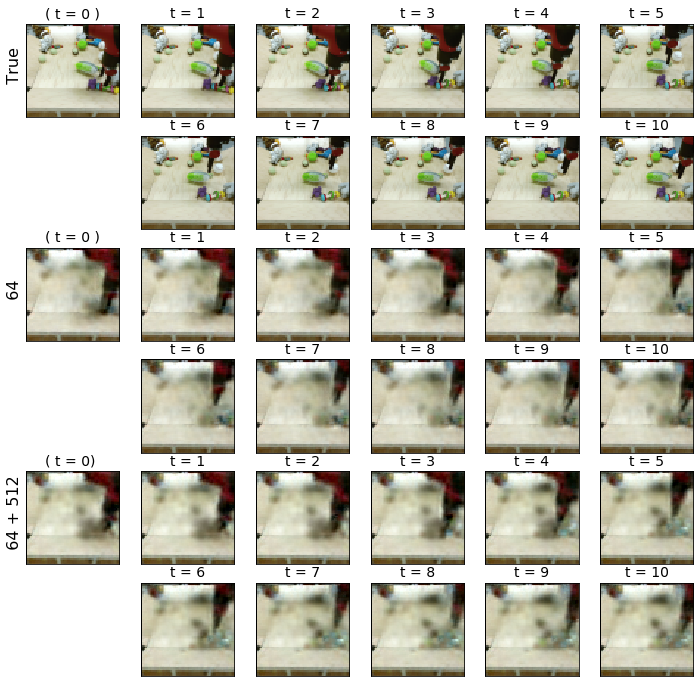
\includegraphics[clip, width=0.63\linewidth]{./figures/pred_c.png}
    \label{fig:pred_c}}
    \\
    \subfloat[]{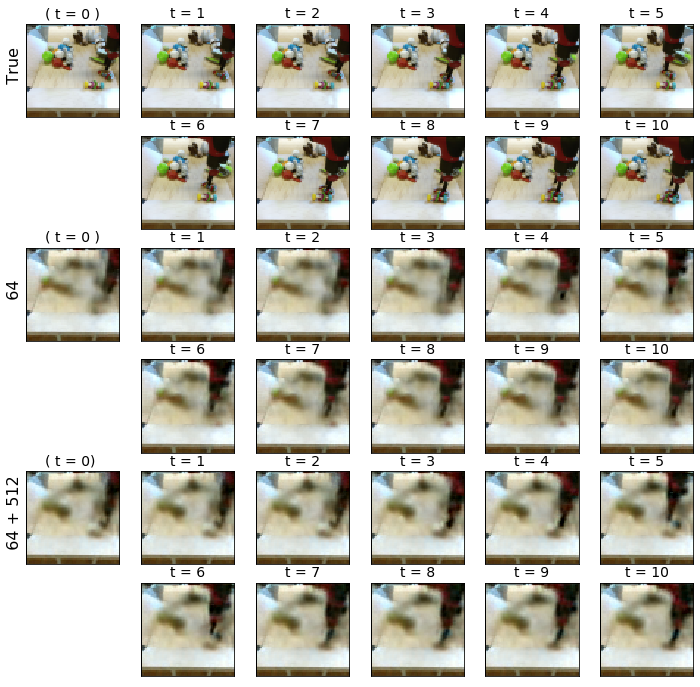
\includegraphics[clip, width=0.63\linewidth]{./figures/pred_d.png}
    \label{fig:pred_d}}
    \caption[映像予測結果2]{映像予測結果2.「True」が正解映像,「64」がベースライン(64)での予測結果,「64 + 512」が提案手法(64 + 512)での予測結果を示す.また$t = 0$は初期状態の推論時に与えられるフレーム.}
    \label{fig:compare_cd}
\end{figure}

\begin{figure}[tbp]
    \begin{center}
        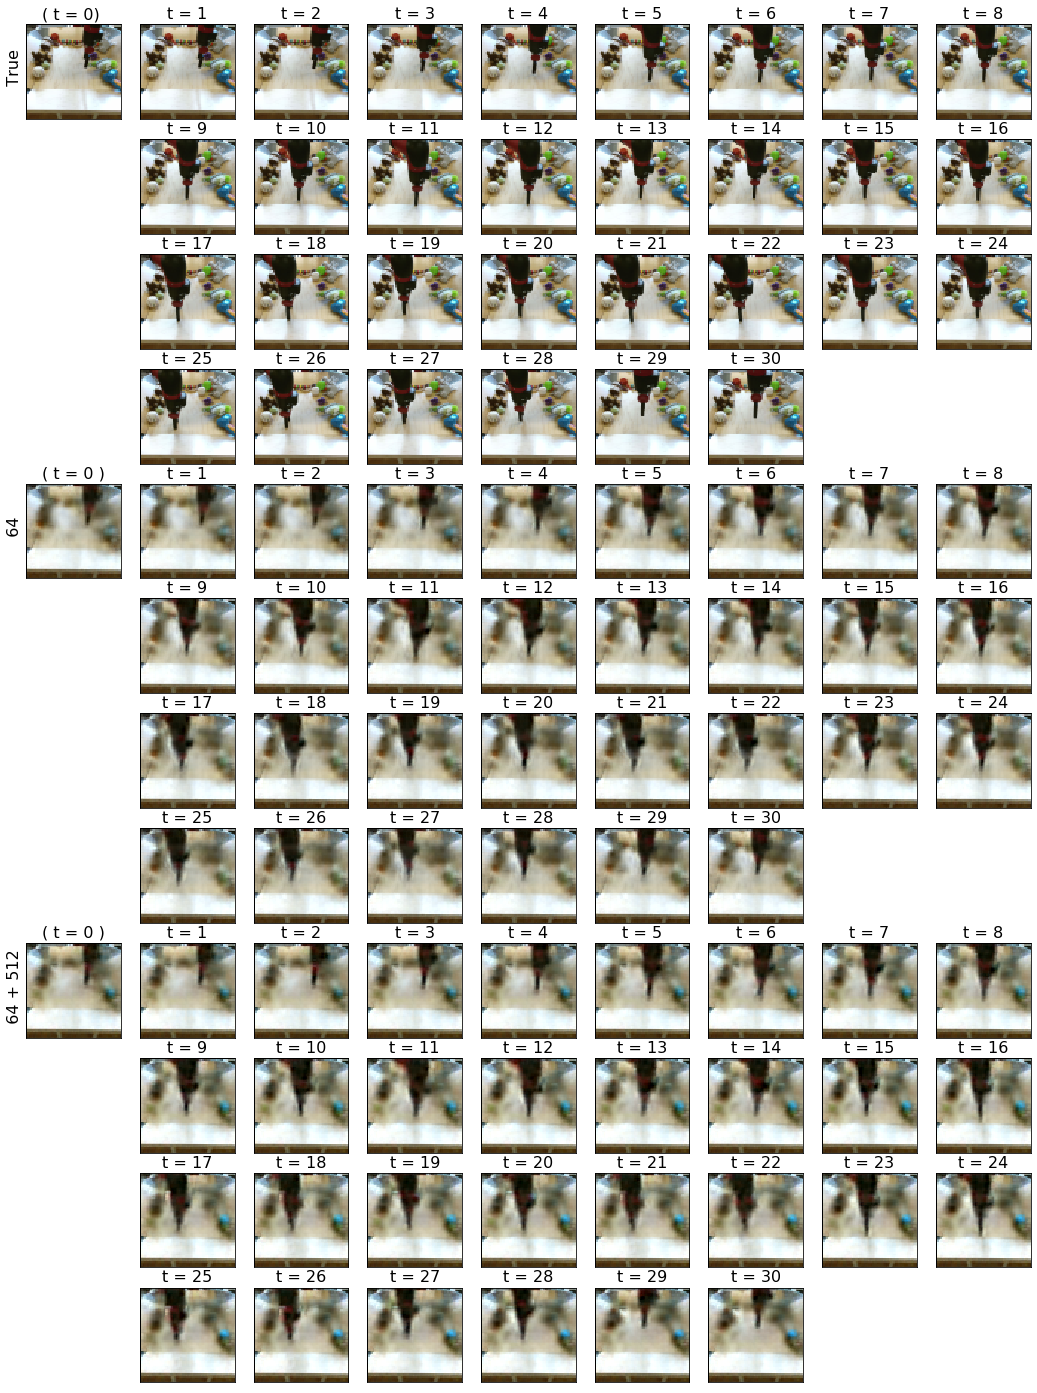
\includegraphics[width=0.95\linewidth]{./figures/pred_long.png}
        \caption[30フレームの予測結果の比較]{30フレームの予測結果の比較.「True」が正解映像,「64」がベースライン(64)での予測結果,「64 + 512」が提案手法(64 + 512)での予測結果を示す.また$t = 0$は初期状態の推論時に与えられるフレーム.}
        \label{fig:pred_long}
    \end{center}
\end{figure}

% 次元の大きさ ~ 情報量の大きさ 

% 高次元の潜在変数を用いたい場合は今回の手法は有効である.

% 三階層にしても学習は進むが,階層にして潜在変数の次元を大きくするだけでは性能の向上に限界がある.
\chapter{考察}
\label{chap:discussion}

\section{本研究の貢献}

\section{今後の課題}
\subsection{転移学習}
環境のダイナミクスとして、普遍的な物理法則を一部獲得していると考えられることから、様々なタスクで
特に階層的なモデルでは、低次元のstateに大域的な物理法則に関するダイナミクス、高次元のstateに比較的表面的なダイナミクスを
獲得していると考えられ、普遍的な環境の多少の変化には

\section{社会応用}
\subsection{実機ロボットへの応用}

\subsection{物理シミュレーションの近似}
本研究で扱った深層学習ベースの行動条件付き映像予測では物理現象の結果として観測されるデータの近似を行うが、これは物理現象の近似という意味で現行の物理シミュレーションソフトウェアと同じことを行っていると解釈ができる。現在、物理シミュレーションの手法としては、既知の様々なスケールの物理法則を記述し微小時間・微小空間単位で逐次的に各領域の状態を計算し全体の結果を予測することが一般的である。しかしこのアプローチは、物理法則が既知である必要があり、また複雑な物理法則に対しては予測に膨大な時間がかかりリアルタイムに予測ができないという問題がある。例えば[]は、蕎麦にオイスターソースをかけて混ぜる物理シミュレーションを扱っているが、1フレームごとの見た目はとてもリアルなものの物理現象としては以前不自然な部分があり、さらに30fpsで1秒の予測をするのに29時間かかると報告している.現行の物理演算ベースの映像予測に対し深層学習ベースの映像予測は、物理法則の正しさや多視点から見た際の一貫性が保証できないなど機能として制限は多いものの、一度学習すればリアルタイムで予測を行うことができる。また必要なデータを集めることで機能の制限を解消することもできるはずである.

これからの人工知能の研究には仮想現実環境の開発が欠かせない。これは、昨今強化学習やロボット学習の分野で相次いて世界中の研究機関が学習用のシミュレーション環境[Meta world, control suit, RLBench]を開発し公開していることからも伺えるが、物理的なタスクを解けるよう学習するには実環境では危険であったり学習の並列化が難しいからである。自ら動いてものとの相互作用を繰り返す中で身体性また予期しなかった、身体性という観点から.

てと考えているが、物理演算ベースと深層学習ベースの物理シミュレーションの融合、あるいは深層学習ベースによる代替を研究していくことも重要になるだろう.


\chapter{結論}
\label{chap:conclusion}

本論文では,実機ロボットへの応用を見据えて深層状態空間モデルを用いた映像予測について取り上げた.まず深層強化学習などで用いられているシンプルな深層状態空間モデルでは複雑な環境を扱う問題設定に上手くスケールしない問題を示した.その上で深層状態空間モデルの状態表現の階層性を明示的にモデル化した提案手法によってより高次元の状態表現を扱えるようにし,さらに映像予測の性能が向上することを示した.
実験では,定性的な大きな優位性は示せなかったものの,高次元の状態変数を用いた学習を可能にしたことは深層状態空間モデルの大きな問題を克服したと言える.これにより,これまで映像予測の分野では実機ロボットへの応用上の制約が多いにも関わらず自己回帰的なモデルの研究が主流であったが,状態空間モデルベースの手法が見直されるきっかけになるかもしれない.

第\ref{chap:discussion}章では展望として深層状態空間モデルの研究の方向性を複数上げたが,これらの研究をすすめることによってより高性能な予測が可能になり,また実機への応用の可能性も高められると考える.さらに応用の例として,映像予測の実機応用に加え,新たな物理シミュレーションの近似アプローチと新たなロボット学習のあり方の可能性について述べた.この二つの応用例は現段階では可能性の話に過ぎず実現可能かは定かでないがどちらも実現すれば社会的な価値は大きいと考えられるので,今後も慎重に研究を継続していきたい.

\chapter*{謝辞}
\label{chap:acknowledgments}
\addcontentsline{toc}{chapter}{謝辞}
本論文を作成するにあたり,多くの方々にご協力をいただきました.

松尾豊教授には,私が取り組みたい研究テーマについて興味を持っていただき,研究アイディアの方向性や可能性について多くのアドバイスをいただきました.当初私がやると言った内容の多くは展望や応用の節で触れるに留まってしまいましたが,今後また時間をとって研究し形にしたいと考えています.

岩澤有祐特任助教には具体的な研究内容を決める段階から執筆までサポートしていただき,岩澤特任助教の的確な研究方針のアドバイスがあって辛うじて卒業論文をまとめることができました.先行研究や提案手法の実装にあたっては,今回使わせて頂いた深層生成モデルのライブラリを開発している特任研究員の鈴木雅大さん,博士課程の金子貴輝さん,学科後輩の原田憲王くんにたいへんお世話になりました.また実験がうまく行かなかった際には博士課程の阿久澤圭さん,修士課程の谷口尚平さんに実装上のアドバイスを多くいただき,研究を進めることができました.修士課程の松嶋達也さんには毎日のように面倒を見ていただき,研究の仕方から研究生活についてまで非常に多くのことを学ばせていただいたきました.特任研究員の河野慎さんは私に学会参加を勧めて下さり,発表を目標に本研究を大きく加速させることができました.研究室のサーバーチームの皆様には日頃からお世話になり,お陰様で不自由なく実験を進めることができました.皆様本当にありがとうございました.

最後に,研究室配属から一年の間,あらゆる面でサポートをしてくださった松尾研究室の皆様に御礼申しあげて,謝辞とさせて頂きます.

\begin{flushright}
東京大学工学工学部システム創成学科\\
知能社会システムコース\\
松尾研究室学部 4年\\
平成31年2月 近藤生也\\
\end{flushright}
\bibliography{references}
\end{document}
